\section{Introduction}
\label{sec:introduction}

Local quantum walks and quantum cellular automata (QCA) provide exact unitary
models in which finite-range update rules approach relativistic wave
equations.  Product-form Dirac walks have rigorous observational convergence
results \citep{Arrighi2014DiracWalk}.  A one-dimensional direct Dirac QCA was
derived from homogeneity, locality, unitarity, parity, and time-reversal
requirements, and was compared with continuum Dirac evolution through unitary
channel discrimination \citep{Bisio2015QuantumFieldQCA,
DAriano2014InformationPrinciples}.  Zitterbewegung and scattering from a
position-dependent potential are likewise established for that direct family
\citep{Bisio2013DiracQCADynamics}.  The existence of the direct automaton, its
low-momentum Dirac limit, and those dynamical phenomena are therefore not the
novelty of the present work.

The open methodological question addressed here is narrower and, in a
different sense, more demanding.  Suppose a target theory is represented not
by visual resemblance or one asymptotic expansion, but by a frozen collection
of operational roles: a uniform evolution bound on a declared input sector,
fixed encoding and intervention maps, fixed measurement witnesses, causal and
symmetry requirements, explicit resources, and independent numerical
reconstruction.  Can two separately specified finite local updates satisfy the
same bounded role after each test has been fixed and its confirmation cases
withheld?

This formulation separates three questions that are often collapsed.
First, an \emph{analytic construction} can establish exact locality,
unitarity, symmetry, or a formal continuum expansion.  Second, a
\emph{registered operational test} can establish that a particular finite
construction meets declared error and intervention criteria on a bounded
domain.  Third, a \emph{structural breadth claim} asks whether mechanisms that
remain distinct under a declared equivalence relation pass the role.  Passing
one construction does not answer the third question, while two frozen
specifications that are related by a change of frame do not establish an
architecture-wide theorem.

We implement the operational comparison for two radius-one updates.  The first is
an ordered product of a scalar phase, an on-site mass mixer, and a two-layer
conditional transport circuit.  The second uses the established direct Dirac
QCA one-particle law, but declares and audits a full-space hard-core-qubit
localization comprising an edge scatter and an on-site routing SWAP.  As
registered, the updates have different gate partitions and finite-step
signatures: the product walk has a leading Lie--Trotter ordering error, while
the direct free update has an even-in-step effective-generator correction.
Their one-excitation blocks are nevertheless related by an exact half-cell
time-frame conjugacy and gate fusion, which we make explicit below.  We
therefore claim only enumerative coverage at the registered-specification
level, not two algebraically independent dynamical families or an architecture
class.

The evidence was produced sequentially: the product result completed before
the direct follow-on was frozen.  This is not a jointly frozen two-arm trial.
It is prospective within each registration.  For each update, candidate law,
target, maps, scenarios, states, metrics,
thresholds, numerical precision, and stopping rule were content-sealed before
registered outcomes.  Development was evaluated as one indivisible batch.
Only a committed development pass accepted by an algorithmically separate
reconstruction could open a fresh, indivisible, single-use confirmation
batch.  Confirmation is not treated as a large statistical sample: the
primary certificate is uniform over a fixed 18-dimensional input sector, and
the held-out intervention schedules provide a non-algebraically-implied test
of the frozen construction.

The resulting contribution is fourfold:

\begin{enumerate}
  \item one common bounded Dirac role is made executable through fixed
  encoding, intervention, and readout maps rather than trajectory inspection;
  \item two separately specified local updates are tested under separately
  frozen, realization-appropriate convergence gates;
  \item declared circuit clocks, causal support, arithmetic precision, and
  algorithmically separate reconstruction are reported as part of the
  evidence; and
  \item the registered evidence is paired with explicit time-frame,
  compilation, global-spectrum, lift, and post-result audit boundaries.
\end{enumerate}

The four counted v0.4 stage ledgers recorded positive development and
single-use confirmation classifications.  A post-result audit withdrew one shared empirical
$\pi$-sector reducer from both primary and replay evidence while preserving its
separate pre-outcome analytic bound.  The supported conclusion is consequently one of
\emph{qualified constructive sufficiency for the intact shared bounded core
across two registered update specifications}.
It is not the first operational comparison between a QCA and the Dirac theory;
it is a sequential, separately prospective, multi-criterion comparison across
two finite updates with explicit resource and provenance controls.

\begin{figure}[t]
  \centering
  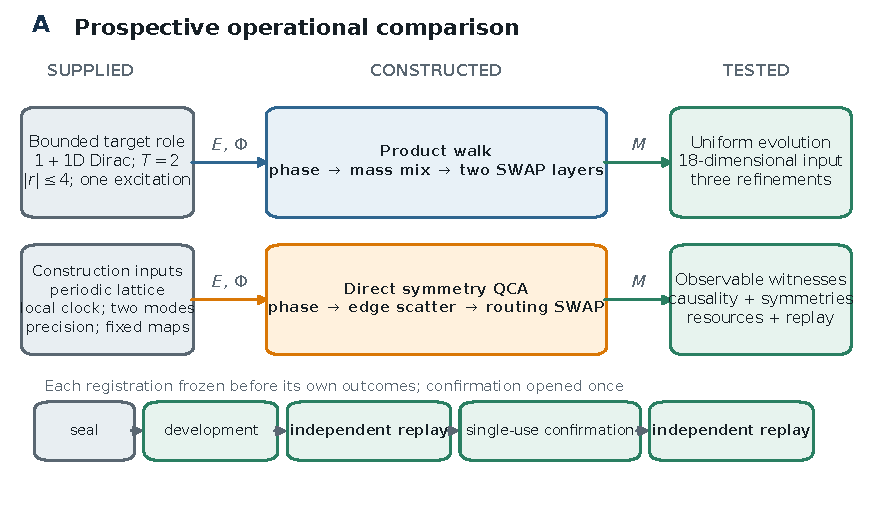
\includegraphics[width=\linewidth]{quantum_dirac_paper/figures/generated/fig01_construction_map.pdf}
  \caption{\textbf{Frozen operational-comparison contract (\conceptual).}
  The bounded target, quantum substrate, clock, constants, precision, maps,
  interventions, and gates are supplied.  The constructed objects are two
  separately registered local updates.  Both are tested with a uniform
  evolution bound, observable witnesses, structural requirements, resource
  accounting, and an algorithmically separate replay, subject to the shared
  $\pi$-reducer exception in Sec.~\ref{sec:post-result-audit}.  The arrows denote
  operational maps, not a derivation of the Dirac equation or quantum theory.}
  \label{fig:construction-map}
\end{figure}
